%!TEX root = ../masters_thesis.tex

\chapter{The Hivent Model} % (fold)
\label{cha:the_hivent_model}

The task of this thesis is to model, visualize and edit the development of countries in time and space in a HGIS. Before the system itself can be developed, the underlying data model has to be fixed. This is the purpose of this chapter.

In section \ref{sec:spatio_temporal_data_models}, different spatio-temporal data models were introduced to solve this problem. The \emph{Snapshot Model} was seen as unsuitable for the problem space. \emph{Simple Time-Stamping} is helpful to link countries to their history, but the method does not explicitly model historical changes, which is desireable. For that purpose, the idea of the \emph{Event-Based Spatio-Temporal Data Model} was developed, but since it only works for raster data, it is also not suitable for this thesis. This problem is solved in the \emph{History Graph Model}. Additionally, the introduced temporal changes allow to represent historical changes and their influences on geographic entities directly in the model. Finally, the \emph{Three-Domain Model} introduces a helpful concept to separate the spatial, temporal and thematic dimension of a spatio-temporal entity.

The \emph{Hivent Model} developed in this thesis is constructed from components of some of these models: An Event-Based Spatio-Temporal Data Model organized according to the Three-Domain Model, using Simple Time-Stamping for the spatial entities, supporting vector data and visualization on a History Graph.

In the first section of this chapter, the main elements of the Hivent model are introduced. Afterwards, the preconditions are defined. The next section explains the Historical Geographic Operations that are used to change countries in time and space. The data structures used to organize the elements of the model are illustrated in the last section.
% The chapter closes with an informal proof that the model is approproate.
% -> no, this will be part of the evaluation

% ==============================================================================
\section{Elements} % (fold)
\label{sec:elements}

The main elements of the the model are the \emph{Hivent}, representing an historically significant happening and the \emph{Area}, an abstract entity on a map with a name and a territory. An \emph{Historical Change} is part of one Hivent and manipulates the history of one or more Areas.

% - - - - - - - - - - - - - - - - - - - - - - - - - - - - - - - - - - - - - - -
\paragraph{Hivents} % (fold)
\label{par:hivent}

are the main organizing element of the data model. The word is an acronym for \emph{\textbf{Hi}}storical e\emph{\textbf{vent}}. It represents a significant happening in history at one specific time point, e.g. a treaty, bill or declaration. In this domain, the focus is on events that influence the geopolitical situation on Earth. That means, they introduce historical changes at their point in history. An Hivent has five different attributes:

\begin{compactenum}
  \item The \emph{name} of the Hivent.
  \item A textual \emph{description} of the topic of the Hivent.
  \item The point in time, identified by the Hivent \emph{date}.
  \item The Hivent \emph{location}.
  \item The \emph{historical changes} resulting from the Hivent.
\end{compactenum}

% paragraph hivent (end)

% - - - - - - - - - - - - - - - - - - - - - - - - - - - - - - - - - - - - - - -
\paragraph{Areas} % (fold)
\label{par:area}

are the the visible entities on the map. They are an abstract representation of one identical current or historical country. The model can easily be extended to the history of states, provinces or regions. Therefore, from now on the term \emph{political unit} instead of \emph{country} is used to describe the object in the real world that is modeled by an Area.

Each Area has a \emph{short name}, e.g. ``Germany'', and a \emph{formal name}, e.g. ``Federal Republic of Germany''. The main spatial dimension of the data model is the Areas \emph{territory}, represented by a polypolygon. It is a set of weakly simple polygons, because the model has to support enclaves and exclaves. The polylines of the polygons represent the borders of the political unit. A polyline consists of an ordered set of points, representing the border points.

An Area can change over time. Throughout its lifetime, it is created at some point $t_s$, then its territory and short name can change multiple times $t_i: t_s < t_i$ and at some point $t_e: t_s < t_i < t_e$ it ceases. Since all changes in this model are sudden, there are only two possible states an Area can be in: It is \emph{active}, if at the current time point it is historically existing and it is \emph{inactive} if it does not. Each area is uniquely identified by its formal name. That means, the short name can change, but as soon as the formal name of an area changes (e.g. ``German Empire'' to ``Federal Republic of Germany''), it is considered a ``new'' Area.

\begin{figure}[H]
  \centering
  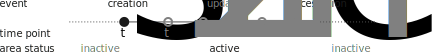
\includegraphics[width=0.8\textwidth]{graphics/hivent_model/area_states}
  \caption{Three types of changes to Areas, two different area states}
  \label{fig:area_states}
\end{figure}

% paragraph area (end)

% ------------------------------------------------------------------------------
\paragraph{Historical Changes} % (fold)
\label{par:historical_changes}

influence the development of an Area over time. They can create new Areas, update their territory or name and cease them. Each Historical Change belongs to exactly one Hivent, inheriting its time point at which the change happens.  The change is described by a Historical Geographic Operation introduced in section \ref{sec:historical_geographic_operations}.

% paragraph historical_changes (end)

% ==============================================================================
\section{Preconditions} % (fold)
\label{sec:preconditions}

\begin{quoteit}
In the beginning God created the heavens and the Earth \\
Now the Earth was formless and empty [...] \\
And God said, “Let there be light” --- and there was light.
\end{quoteit}
\hfill -- Genesis 1:1, The First Book of Moses, Old Testament

The spatio-temporal system has to be initialized at some point. It is based on a set of trivial axioms stated in this section. Each Area in the system is located directly on the surface of the Earth. While the surface is curved, as explained in sections \ref{sub:model_of_geographical_space} and \ref{sub:presentation_of_geographic_space}, it can be projected on a two-dimensional map.

\vspace{-1.0em}
\newtheorem{invariant_surface}[assicounter]{Axiom}
\begin{invariant_surface}
\label{axm:invariant_surface}
  The Earth's surface has an invariant area size, i.e. it does not change over time.
\end{invariant_surface}

This axiom sets the spatial foundation of the system: a constant dimension of the map. The basis of the temporal part of the system is introduced in the next three axioms:

\vspace{-1.0em}
\newtheorem{initial_configuration}[assicounter]{Axiom}
\begin{initial_configuration}
\label{axm:initial_configuration}
  The spatio-temporal system has an initial state at time point $t_0$. At this initial state, there exists exactly one Area, denoted by $\Omega$ and referred to as the \emph{universe} Area. It has no name and its territory covers the whole surface of the Earth.
\end{initial_configuration}

\vspace{-1.5em}
\newtheorem{historical_change}[assicounter]{Axiom}
\begin{historical_change}
\label{axm:historical_change}
  At each time point $t_i \geq t_0$ an Historical Change can be introduced.
\end{historical_change}

\vspace{-1.5em}
\newtheorem{unique_coverage}[assicounter]{Axiom}
\begin{unique_coverage}
\label{axm:unique_coverage}
  At each time point $t_i \geq t_0$ each point on the surface of the Earth is covered by exactly one Area.
\end{unique_coverage}

As it has been defined in section \ref{par:historical_changes}, an Historical Change can create, manipulate and cease Areas on the Earth's surface. According to axoim \ref{axm:unique_coverage}, each change introduced in the system must maintain the spatial integrity on the map. That means, as soon as an Area is created in one territory on the map, the territory that was there before has to cease. Vice versa, if an Area ceases from the map, it has to be replaced with at least one new Area and these new Areas combined have to occupy exactly this same territory.

The first Historical Changes introduced in the system at time point $t_0$ are the creation of all bodies of water, including the oceans and lakes. They are created as Areas with their name and territory which is cut out of $\Omega$. That means, at $t_0$, the map of the world is divided into a set of Areas representing water and $\Omega$, representing land. Land can at any point in time be either \emph{claimed}, i.e. it is currently occupied by the territory of exactly one active Area, or on a contrary be \emph{unclaimed}, i.e. belonging to $\Omega$. It is a subtractive data model, because each Area that is created new will be cut out of $\Omega$.

The borders of a political unit are either \emph{interior}, i.e. bordering another political unit, or a \emph{coastline}, bordering a body of water. This assumption is a concious simplification of the reality: It assumes the territory of a political unit stops at the coastline. Juristically, this is not true, because in line with \cite{UNSeaBorders}, the territory extends in a range of 3 to 12 miles (5 to 20 kilometers) into international waters. This model disregards the sea territory of a political entity to keep the model simple.

In the real world, The name of a political unit changes according to sudden events, e.g. a declaration or a governmental bill. The territory can change either because of a geographical processes, e.g. the Sea Level Rise influencing the change of the coastline, or according to a historical event, e.g. a treaty.

\vspace{-1.0em}
\newtheorem{constant_coastlines}[assicounter]{Assumption}
\begin{constant_coastlines}
\label{axm:constant_coastlines}
  The spatial configuration of the Earth's surface, i.e. land, water and the coastlines, has not changed over time.
\end{constant_coastlines}

While this assumption is obviously wrong, it helps to keep the problem space clear and the Hivent Model simple: it focuses only on discrete historical changes and not on long-term processes. However, it is open to future extensions to account also for geographic changes and international sea borders. In this data model, the temporal behavior of an Area can therefore be described as a \emph{static object that changes according to sudden events}.

% base: Newtons concept of absolute space?
% TODO: topological rule?
% each border has exactly two neighboring Areas
% each Area has at least one neighboring Area

% section preconditions (end)

% ==============================================================================
\section{Historical Geographic Operations} % (fold)
\label{sec:historical_geographic_operations}

Respecting the preconditions, there are five different types of changes that can occur to a set of Areas. They can be expressed with five spatio-temporal operations which are called \emph{Historical Geographic Operations} (HG Operations). Four of them change the identity of a set of Areas and therefore establish historical predecessor-successor-relationships. That means, if one old Area is replaced by one new Area, the old Area is the historical predecessor of the new Area and vice versa the new Area is the successor of the old Area.
% Historical relationships are only noted in one direction (predecessor), but are always valid also in the other direction (successor).

\begin{description}
  \item[UNI -- Unification]
  A set of old Areas unifies to ome new Area. The old Areas cease, becoming the historical predecessors of the new Area. This new Area receives a new name and its territory is the union of the territories of the old Areas. \\
  \begin{footnotesize}
    In 1922, the Russian SFSR, the Transcaucasian SFSR, the Ukrainian SSR and the Byelorussian SSR unified and formed the Union of Soviet Socialist Republics (USSR).
  \end{footnotesize}
  \item[INC -- Incorporation]
  One or more old Areas are incorporated into another Area that stays active. Its territory is enlarged by the union of the territories of the old Areas. The old Areas are historical predecessors of the new Area. \\
  \begin{footnotesize}
    In 1990, the territory of the German Democratic Republic (East Germany) became part of the Federal Republic of Germany (West Germany). Although this event is known as the \emph{German Reunification}, it is historically an incorporation of East Germany into West Germany \cite{incorporationEastWestGermany}.
  \end{footnotesize}
  \item[SEP -- Separation]
  As the inverse of unification, one old Area is preceded by multiple new Areas. Each new Area gets a new name, receives a part of the territory of the old Area, and the old Area as its only historical predecessor. \\
  \begin{footnotesize}
    In 1993, the Czech and Slovak Federal Republic, commonly known as Czechoslovakia, dissolved into present-day Czech Republic and Solvak Republic, creating two new countries.
  \end{footnotesize}
  \item[SEC -- Secession]
  As the inverse of incorporation, one or more new areas are ceded from a previously exising area that stays active. Each new Area gets a new name, receives the previously existing Area as the only historical predecessor and a part of its territory. \\
  \begin{footnotesize}
    In 2008, the Republic of Kosovo declared independence from Serbia and has since then partially received international recognition. Unlike in the case of separation, Serbia stays as country, keeping its name, but ceding a part of its territory to Kosovo.
  \end{footnotesize}
  \item[NCH -- Name Change]
  An Area changes its short name but preserves its identity. \\
  \begin{footnotesize}
    A recent change happened on 5. May 2016: The cabinet of Czech Republic approved that the country will now offically be called ``Czechia''. The formal name stays ``Czech Republic''.
  \end{footnotesize}
\end{description}

% - - - - - - - - - - - - - - - - - - - - - - - - - - - - - - - - - - - - - - -
\begin{table}[H]
\begin{center}
\begin{tabular}{m{0.75cm} m{2.5cm} m{2.5cm} m{2.0cm} m{2.5cm}}
  \toprule
  & operation
  & \multicolumn{1}{c}{visualization}
  & \multicolumn{1}{c}{\pbox{2.5cm}{historical\\relationship}}
  & \multicolumn{1}{c}{territory} \\

  \midrule
  \texttt{UNI} & Unification & \raisebox{-0.25\height}
  {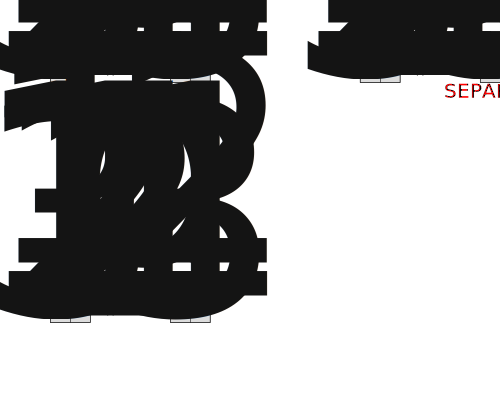
\includegraphics{graphics/hivent_model/operations/UNI}} &
  $ A_i \leftrightarrow_H B $ &
  $ B^T = \cup_{i=1}^{n} A_i $ \\

  \midrule
  \texttt{INC} & Incorporation & \raisebox{-0.25\height}
  {\includegraphics{graphics/hivent_model/operations/INC}} &
  $ A_i \leftrightarrow_H A_0 $ &
  $ A_0^T = \cup_{i=1}^{n} A_i $ \\

  \midrule
  \texttt{SEP} & Separation & \raisebox{-0.25\height}
  {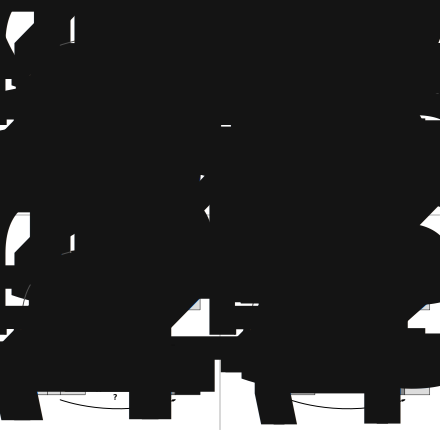
\includegraphics{graphics/hivent_model/operations/SEP}} &
  $ A \leftrightarrow_H B_i $ &
  $ B_i^T \cap A^T = B_i^T $ \\

  \midrule
  \texttt{SEC} & Secession & \raisebox{-0.25\height}
  {\includegraphics{graphics/hivent_model/operations/SEC}} &
  $ A_i \leftrightarrow_H A_0 $ &
  $ B_i^T \cap A^T = B_i^T $ \\

  \midrule
  \texttt{NCH} & Name Change & \raisebox{-0.25\height}
  {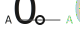
\includegraphics{graphics/hivent_model/operations/NCH}} &
  $ \emptyset $ &
  $ \emptyset $ \\

  \bottomrule
\end{tabular}
\caption{Overview about the five HG Operations}
\label{tab:historical_geographic_operations}
\end{center}
\end{table}

% - - - - - - - - - - - - - - - - - - - - - - - - - - - - - - - - - - - - - - -
\paragraph{Functional description} % (fold)
\label{par:functional_description}

Each HG Operation can be described by a mathematical function. The following symbols are used in the equations:

\begin{addmargin}[1em]{0em}
\begin{tabbing}
  symbolxx \= description1xx \= description2 \kill
  $A$ \> set of old Areas that were active before the Historical Change \\
  $B$ \> set of new Areas that are created in the Historical Change \\
  $n:$ \> $n \in \mathbb{N}, n>0$ \> total number of old respectively new Areas \\
  $i:$ \> $i \in [\textbf{1} .. n]$ \> iterator for the current old respectively new Area \\
  $A_0/B_0$ \>    the first old respectively new Area ($i \geq 1 \Rightarrow$ not $A_i/B_i$~!) \\
  $A_i/B_i$ \>    the current old respectively new Area ($i \geq 1 \Rightarrow$ not $A_0/B_0$~!) \\
  $A_i^T/B_i^T$ \>the new territory of the current Area (a polypolygon) \\
  $A_i^N/B_i^N$ \>the new name of the current Area (short and formal name) \\
\end{tabbing}
\end{addmargin}

\vspace{-2.5em}
\begin{align*}
  (B_0)                       &= UNI([A_1 .. A_i .. A_n], B_0^N) \\
  (A_0)                       &= INC(A_0, [A_1 .. A_i .. A_n]) \\
  ([B_1 .. B_i .. B_n])       &= SEP(A_0, [[B_1^T, B_1^N] .. [B_i^T, B_i^N] .. [B_n^T, B_n^N]]) \\
  (A_0, [B_1 .. B_i .. B_n])  &= SEC(A_0, A_0^T, [[B_1^T, B_1^N] .. [B_i^T, B_i^N] .. [B_n^T, B_n^N]]) \\
  (A_0)                       &= NCH(A_0, A_0^N)
\end{align*}


% paragraph functional_description (end)

% - - - - - - - - - - - - - - - - - - - - - - - - - - - - - - - - - - - - - - -
\paragraph{Pseudocode description} % (fold)
\label{par:pseudocode_description}

of the HG operations in an object-oriented manner. The existance of a class \texttt{Area} is assumed. Each \texttt{Area} object has the following member variables: a \texttt{name}, a \texttt{territory} and a list of historical \texttt{predecessors} and \texttt{successors}. Single capital letter variables (\texttt{A}/\texttt{B}) denote arrays of \texttt{Area} objects. Variables with a capital letter followed by a number or lowercase letter (e.g. \texttt{B0}) are single \texttt{Area} objects.

\begin{minipage}[t]{0.47\textwidth}
\begin{lstlisting}[language=pseudocode,
  caption=Unification]
FUNCTION UNI(A, B0_name)
  # create new territory
  B0_territory = NEW Geometry # empty
  FOREACH Ai IN A
    B0_territory.union(Ai.territory)
  # create new area
  B0 = NEW Area(B0_name, B0_territory)
  # establish historical relationships
  FOREACH Ai IN A
    Ai.successors.add(B0)
    B0.predecessors.add(A1)
  # return new area
  RETURN B0
\end{lstlisting}
\end{minipage}    % N.B. the % is very important
\hspace{3.0em}    % N.B. this must go in this line, no blank lines !!!
\begin{minipage}[t]{0.47\textwidth}
\begin{lstlisting}[language=pseudocode,
  caption=Incorporation]
FUNCTION INC(A0, A)
  # update old area with new territory
  temp_terr = NEW Geometry # empty
  FOREACH Ai IN A
    temp_terr.union(Ai.territory)
  A0.territory = temp_terr
  # establish historical relationships
  FOREACH Ai IN A
    Ai.successor.add(A0)
    A0.predecessor.add(A1)
  # return new area
  RETURN A0
\end{lstlisting}
\end{minipage}

\begin{minipage}[t]{0.47\textwidth}
\begin{lstlisting}[language=pseudocode,
  caption=Separation]
FUNCTION SEP(A0, B_data)
  # create each new Area
  B = []
  FOREACH Bi_data in B_data
    B.add(NEW Area(
      Bi_data.name, Bi_data.territory)
    )
  # establish historical relationships
  FOREACH Bi IN B
    A0.successors.add(Bi)
    Bi.predecessors.add(A0)
  # return new areas
  RETURN B

\end{lstlisting}
\end{minipage}    % N.B. the % is very important
\hspace{3.5em}    % N.B. this must go in this line, no blank lines !!!
\begin{minipage}[t]{0.47\textwidth}
\begin{lstlisting}[language=pseudocode,
  caption=Secession]
FUNCTION SEC(A0, A_territory, B_data)
  # update old area with new territory
  A0.territory = A_territory
  # create each new Area
  B = []
  FOREACH Bi_data in B_data
    B.add(NEW Area(
      Bi_data.name, Bi_data.territory)
    )
  # establish historical relationships
  FOREACH Bi IN B
    A0.successors.add(Bi)
    Bi.predecessors.add(A0)
  # return old and new areas
  RETURN [A0, B]

\end{lstlisting}
\end{minipage}

\vspace{-1.5em}
\begin{minipage}[t]{0.47\textwidth}
\begin{lstlisting}[language=pseudocode,
  caption=Name Change]
FUNCTION NCH(A0, A_name)
  # update old area with new name
  A0.name = A_name
  # return updated area
  RETURN A0

\end{lstlisting}
\end{minipage}

% paragraph pseudocode_description (end)

% section historical_geographic_operations (end)

% ==============================================================================
\subsection{Data Structures} % (fold)
\label{sub:data_structures}

execute function for all operations the same

\begin{lstlisting}[language=pseudocode,
  caption=class HGOperation]

## member variables
update_area = {
  area :          null  # Area
  old_name :      null  # AreaName
  new_name :      null  # AreaName
  old_territory : null  # AreaTerritory
  new_territory : null  # AreaTerritory
}
old_areas = []          # Area
new_areas = []          # Area

## main function
FUNCTION execute(direction)

  # check if one area is updated
  IF update_area.area
    IF update_area.area.new_name
      IF direction IS 1 # forward change
        update_area.area.name = new_name
      ELSE              # backward change
        update_area.area.name = old_name
    IF update_area.area.new_territory
      IF direction IS 1 # forward change
        update_area.area.territory = new_territory
      ELSE              # backward change
        update_area.area.territory = old_territory
    update_area.area.update()

  # hide old areas
  FOREACH old_area IN old_areas
    IF direction IS 1 # forward change
      old_area.hide()
    ELSE              # backward change
      old_area.show()

  # show new areas
  FOREACH new_area IN new_areas
    IF direction IS 1 # forward change
      new_area.show()
    ELSE              # backward change
      new_area.hide()



\end{lstlisting}


% subsection data_structures (end)

% ==============================================================================

\vspace{2em}
transition to next chapter

% chapter the_hivent_model (end)